\documentclass{standalone}
\usepackage{tikz}
\usetikzlibrary{positioning, arrows.meta, calc, backgrounds, fit, shapes, shapes.multipart, shapes.symbols, backgrounds, fit}

\begin{document}
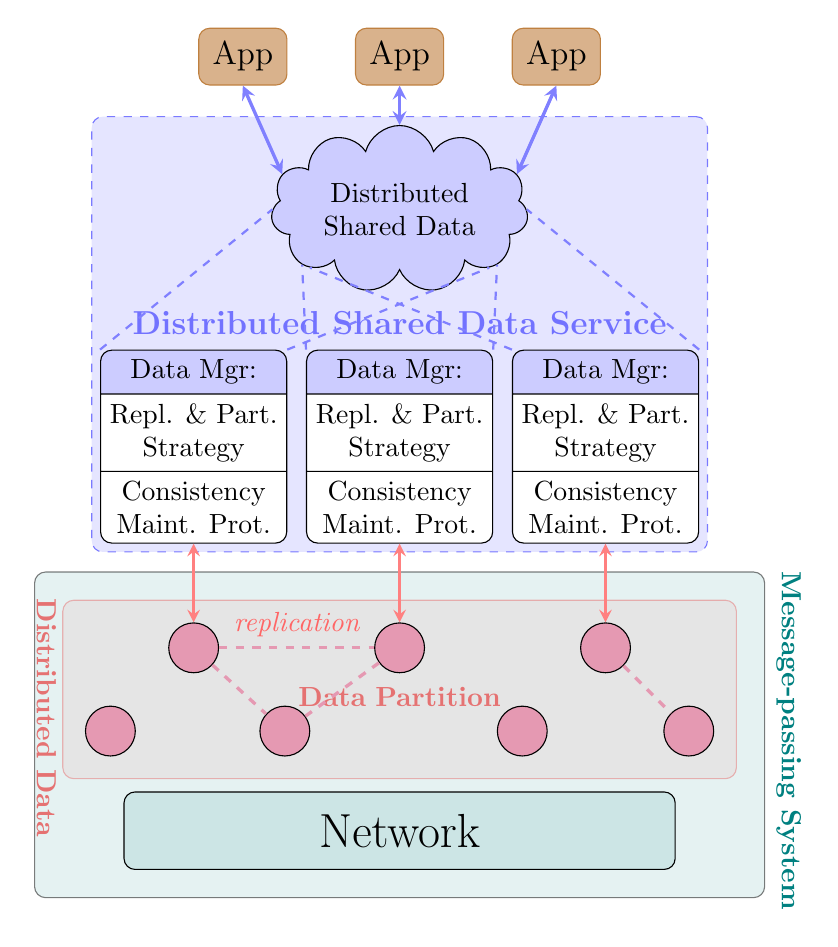
\begin{tikzpicture}[ 
    app/.style = {rectangle, rounded corners, draw = brown, fill = brown!60, font = \large, inner sep = 5pt}, 
    rm/.style = {rounded corners, rectangle split, rectangle split parts = 3, rectangle split part fill = {blue!20, white, white}, draw, align = center},
    app-dsdm/.style = {> = stealth, <->, line width = 1.2pt, draw = blue!50},
    mapping/.style = {dashed, thick, blue!50},
    replica/.style = {rectangle, rounded corners, draw, fill = purple!20, inner sep = 8pt},
	creplica/.style = {circle, draw, fill = purple!40, inner sep = 0pt, 
		minimum size = 18pt},
	replication/.style = {dashed, purple!40, very thick},
    rm-replica/.style = {> = stealth, <->, line width = 1pt, draw = red!50},
    network/.style = {rectangle, rounded corners, draw, fill = teal!20, minimum width = 7.0cm},
    mp/.style = {> = stealth, <->, line width = 1pt, draw = teal!50}]

  % dsdm: distributed shared data model
  \node[name = dsdm, cloud, cloud puffs = 11, draw, fill = blue!20, aspect = 2, 
  	minimum width = 2.00cm, minimum height = 1.00cm, align = center] {Distributed\\Shared Data};

  % apps
  \def\APPDIST{0.50}
  \def\APPSHIFT{0.50}
    % app1 above dsdm.puff 1
  \node[app, above = \APPDIST cm of dsdm.puff 1] (app1) {App};
    % app3 above dsdm.puff 3
  \path let \p1 = (dsdm.puff 3), \p2 = (app1) in node[app, xshift = -\APPSHIFT cm] (app3) at (\x1, \y2) {App};
    % app10 above dsdm.puff 10
  \path let \p1 = (dsdm.puff 10), \p2 = (app1) in node[app, xshift = \APPSHIFT cm] (app10) at (\x1, \y2) {App};

  % apps <-> dsdm
    % app1 <-> dsdm.puff 1
  \draw[app-dsdm] (app1.south) to (dsdm.puff 1);
    % app3 <-> dsdm.puff 3
  \draw[app-dsdm] (app3.south) to (dsdm.puff 3);
    % app10 <-> dsdm.puff 10
  \draw[app-dsdm] (app10.south) to (dsdm.puff 10);

  % rm: replica manager
  % rml: rm label
  \newcommand{\rml}{Data Mgr: 
	\nodepart{second} Repl. \& Part.\\Strategy 
  	\nodepart{third} Consistency\\Maint. Prot.
  }

  \def\RSHIFT{1.00}
    % rm-center below dsdm.south
  \node[rm, below = of dsdm.south] (rm-center) {\rml{}};
    % rm-west below dsdm.west
  \path let \p1 = (dsdm.west), \p2 = (rm-center) in node[rm, xshift = -\RSHIFT cm] (rm-west) at (\x1, \y2) {\rml{}};
    % rm-east below dsdm.east
  \path let \p1 = (dsdm.east), \p2 = (rm-center) in node[rm, xshift = \RSHIFT cm] (rm-east) at (\x1, \y2) {\rml{}};

  % rm -- dsdm mapping
  \draw[mapping] (rm-west.north west) to (dsdm.west);
  \draw[mapping] (rm-west.north east) to (dsdm.south east);

  \draw[mapping] (rm-center.north west) to (dsdm.puff 5);
  \draw[mapping] (rm-center.north east) to (dsdm.puff 8);

  \draw[mapping] (rm-east.north west) to (dsdm.south west);
  \draw[mapping] (rm-east.north east) to (dsdm.east);

  % replica
  \def\RDIST{1.00}
  \node[creplica, below = \RDIST cm of rm-center] (replica-center) {};
  \node[creplica, below = \RDIST cm of rm-west] (replica-west) {};
  \node[creplica, below = \RDIST cm of rm-east] (replica-east) {};
  
  \def\RRDIST{0.60}
  \node[creplica, below left = \RRDIST cm and \RRDIST cm of replica-west]
	(replica-west-left) {};
  \node[creplica, below left = \RRDIST cm and 1.00cm of replica-center]
	(replica-center-left) {};
  \node[creplica, below left = \RRDIST cm and \RRDIST cm of replica-east]
  	(replica-east-left) {};
  \node[creplica, below right = \RRDIST cm and \RRDIST cm of replica-east]
  	(replica-east-right) {};

  % replication
  \path (replica-center) edge[replication] (replica-center-left)
	(replica-west) edge[replication] (replica-center-left)
	(replica-west) edge[replication] node[above, red!60]{\it replication} (replica-center)
	(replica-east) edge[replication] (replica-east-right);

  % \node[replica, below = \RDIST cm of rm-center] (replica-center) {Replica};
  % \node[replica, below = \RDIST cm of rm-west] (replica-west) {Replica};
  % \node[replica, below = \RDIST cm of rm-east] (replica-east) {Replica};

  % partition background
  \begin{pgfonlayer}{background}
	\node[draw = red, fill = red!20, semitransparent, rectangle, rounded corners, 
	  inner sep = 8pt, 
	  fit = (replica-west-left) (replica-west) (replica-east) (replica-east-right) 
	  (replica-center-left),
	  align = center, 
	  text opacity = 1,
	  label = {[rotate = -90, xshift = 2.0cm, yshift = -0.20cm] 
		left:{\textcolor{red}{\bf Distributed Data}}}] 
	  (partition-layer) {\textcolor{red}{$\;$\\{\bf Data Partition}}};
  \end{pgfonlayer}

  % rm <-> replica
  \draw[rm-replica] (rm-center) to (replica-center);
  \draw[rm-replica] (rm-west) to (replica-west);
  \draw[rm-replica] (rm-east) to (replica-east);

  % network
  \def\NDIST{1.50}
  \node[network, below = \NDIST cm of replica-center, inner sep = 8pt] (network) 
	{\LARGE Network};

  % mp: message-passing
  % \draw[mp] (replica-center) to (network);
  % \draw[mp] (replica-west) to (replica-west |- network.north);
  % \draw[mp] (replica-east) to (replica-east |- network.north);

  % mps-layer: message-passing system background including replicas and network
  \begin{pgfonlayer}{background}
	\node[draw, fill = teal!20, semitransparent, rectangle, rounded corners, 
	inner sep = 10pt, 
	fit = (partition-layer) (replica-west) (replica-east) (network),
	label = {[rotate = -90, xshift = -2.2cm, yshift = 0.30cm] 
	  right:{\textcolor{teal}{\bf Message-passing System}}}] 
	(mps-layer) {};
  \end{pgfonlayer}

  % dsds-layer: distributed shared data service including rm and dsdm
  \begin{pgfonlayer}{background}
    \node[draw = blue, fill = blue!20, semitransparent, rectangle, rounded corners, dashed, inner sep = 3pt, fit = (rm-west) (rm-east) (dsdm)] (dsds-layer)
	{\textcolor{blue}{\bf \large Distributed Shared Data Service}};
  \end{pgfonlayer}
\end{tikzpicture}
\end{document}
